% Copyright © 2013 Martin Ueding <dev@martin-ueding.de>
%
\input{header.tex}

\usepackage{tikz}
\usetikzlibrary{calc}
\usepackage{xfrac}

\newcommand{\themodul}{physik411}
\newcommand{\thegruppe}{Gruppe 2 -- Florian Seidler}
\newcommand{\theuebung}{7}

\ifoot{\footnotesize{Martin Ueding}}
\ihead{\themodul{} -- Übung \theuebung}
\ofoot{\footnotesize{\thegruppe}}

\def\thesubsection{\thesection\alph{subsection}}

\title{\themodul{} -- Übung \theuebung}
\subtitle{\thegruppe}
\author{
	Martin Ueding \footnote{\href{mailto:mu@uni-bonn.de}{mu@uni-bonn.de}}
}

\hypersetup{
	pdftitle={\themodul {} - Übung \theuebung},
}

\begin{document}

\maketitle

\begin{center}
	\ccbysadetitle
\end{center}

\begin{table}[h]
	\centering
	\begin{tabular}{l|c|c|c|c|c}
		Aufgabe
		& \ref 1
		& \ref 2
		& \ref 3
		& \ref 4
		& $\sum$   \\
		\hline
		Punkte
		& \punkte / 8
		& \punkte / 12
		& \punkte / 14
		& \punkte / 0
		& \punkte / 34
	\end{tabular}
\end{table}

%%%%%%%%%%%%%%%%%%%%%%%%%%%%%%%%%%%%%%%%%%%%%%%%%%%%%%%%%%%%%%%%%%%%%%%%%%%%%%%
%                              Hund'sche Regeln                               %
%%%%%%%%%%%%%%%%%%%%%%%%%%%%%%%%%%%%%%%%%%%%%%%%%%%%%%%%%%%%%%%%%%%%%%%%%%%%%%%

\section{Hund'sche Regeln}
\label 1

Die Schalen werden so besetzt, dass zuerst das s-Orbital, dann das p-Orbital
gefüllt wird, und dort erst die Spins $\uparrow$ und dann $\downarrow$ besetzt
werden. Somit ergeben sich die folgenden Belegungen:

\subsection{Sauerstoff}

Im Sauerstoff, das 8 Valenzelektronen hat, werden die äußeren Schalen wie folgt
besetzt:
\[
	\underset{\text{2s}}{\fbox{$\uparrow \downarrow$}}
	\quad
	\underset{\text{2p}}{\fbox{$\uparrow\downarrow$}\fbox{$\uparrow\downarrow$}\fbox{$\uparrow\phantom\downarrow$}}
\]

Der Gesamtdrehimpuls aus dem p-Orbital sind 4 mal $\ell = 1$, also ist $L = 4$.
Der Spin ist $S = 3 \uparrow + 1 \downarrow = 1$. Somit ist $J = 5$ und $2s + 1
= 3$. Dies ist also $^3\mathrm P_5$ und $\mathrm{[He] 2s^2 \, 2p^4}$.

Wenn allerdings der Gesamtdrehimpuls $L$ die Summe der $m_\ell$ ist, dann ist
$L = 1 + 0 + (-1) + 1 = 1$. Somit wäre der Drehimpuls $J = 2$ und die
spektroskopische Notation $\mathrm{^3P_2}$.

\subsection{Stickstoff}

Besetzung der Schalen:
\[
	\underset{\text{2s}}{\fbox{$\uparrow \downarrow$}}
	\quad
	\underset{\text{2p}}{\fbox{$\uparrow\downarrow$}\fbox{$\uparrow\phantom\downarrow$}\fbox{$\uparrow\phantom\downarrow$}}
\]

Analog zum Sauerstoff, allerdings ist hier noch ein Elektron weniger auf einem
$m_\ell = 0$ Platz. Somit ändert sich nur der Spin auf $S = \sfrac 32$. Ich
erhalte $^4\mathrm P_{\sfrac 32}$ und $\mathrm{[He] 2s^2 \, 2p^3}$.

\subsection{Eifel}

Welches Element soll dies sein?

\subsection{Magnetische Quantenzahl}

$m_J$ gibt die $z$-Komponente des Gesamtdrehimpulses an. Wenn diese entartet
ist, bedeutet dies eine komplette Kugelsymmetrie.

%%%%%%%%%%%%%%%%%%%%%%%%%%%%%%%%%%%%%%%%%%%%%%%%%%%%%%%%%%%%%%%%%%%%%%%%%%%%%%%
%                   Energieskala der diatomischen Moleküle                   %
%%%%%%%%%%%%%%%%%%%%%%%%%%%%%%%%%%%%%%%%%%%%%%%%%%%%%%%%%%%%%%%%%%%%%%%%%%%%%%%

\section{Energieskala der diatomischen Moleküle}
\label 2

\subsection{Rotationsspektrum}

Die Kraft, die zwischen den beiden Stickstoffmolekülen ist, ist deutlich komplexer, als zwischen Kern und Elektron im Wasserstoffatom. Die Molekülorbitale bilden ein sp-Hybridorbital und zwei verbleibende p-Orbitale, die dann in $\sigma$ und $\sigma^*$ bzw. zwei $\pi$-Bindungen eingehen.

Angenommen, der Drehimpuls für das ganze Molekül ist der gleiche gequantelte Drehimpuls wie für das Elektron selbst. Dann gilt:
\[
	E(m) = \frac{L^2}{2m}
\]

Der Massenunterschied zwischen dem Wasserstoffatom und dem Stickstoffmolekül ist $\beth := \mu/m$, ($\beth > 1$). Wenn die Masse um den Faktor $\beth$ größer wird, so wird der Drehimpuls um den Faktor $\beth$ kleiner. Also
\[
	E_{\mathrm N_2} = \beth^{-1} E_{\mathrm H}
\]

\paragraph{Umrechnung der Energie}

Die reduzierte Masse ist:
\[
	\mu
	= \frac{\SI{10}\atomicmassunit \cdot \SI{10}\atomicmassunit}{\SI{20}\atomicmassunit}
	= \SI5\atomicmassunit
\]

Einsetzen der Konstanten gibt:
\[
	\Deltaup E = \SI{1.49}{\milli\electronvolt}
\]

Dies entspricht einer Frequenz von:
\[
	f = \SI{0.36}{\tera\hertz}
\]

Mit $k = \omega/c$ und $\omega = 2 \piup f$ erhalte ich die Wellenzahl:
\[
	k = \SI{75.6}{\radian\per\centi\meter}
\]

\subsection{Schwingungsspektrum}

\fehlt

\paragraph{Umrechnung der Energie}

Bis auf die Wurzel ist die Rechnung die gleiche, wie oben auch.
\[
	\Deltaup E = \SI{143}{\milli\electronvolt}
	\eqnsep
	f = \SI{34.5}{\tera\hertz}
	\eqnsep
	k = \SI{7220}{\radian\per\centi\meter}
\]

\subsection{Elektronische Übergänge}

Das Stickstoffatom ist vergleichbar groß mit dem Wasserstoffatom, und dort sind
die Übergangsenergien einige $\si\electronvolt$. Beim Stickstoff sind die
Übergangsenergien ähnlich groß. Das Stickstoffmolekül ist etwas kleiner als
doppelt so groß, daher sollten die Energien auch in der gleichen Größenordnung
liegen, wenn man das ganze als harmonischen Oszillator betrachtet.

\subsection{Born-Oppenheimer-Näherung}

Die Born-Oppenheimer-Näherung besagt, dass wenn die Kerne langsam genug sind,
sich die Elektronen instantan daran anpassen und wie in einem effektiven
Potential bewegen.

Wenn das Molekül den gleichen Drehimpuls wie die einzelnen Elektronen hat, dann
müssen die Kerne sich um den Faktor $\beth$ langsamer bewegen. Der Abstand ist
vergleichbar zu den Atomen, nur sind die Atomkerne um den Faktor $\beth$
schwerer. Mit $\beth = 9110$ kann durchaus davon ausgegangen werden, dass die
Näherung erfüllt ist.

%%%%%%%%%%%%%%%%%%%%%%%%%%%%%%%%%%%%%%%%%%%%%%%%%%%%%%%%%%%%%%%%%%%%%%%%%%%%%%%
%            Infrarotspektroskopie eines heteronuklearen Moleküls            %
%%%%%%%%%%%%%%%%%%%%%%%%%%%%%%%%%%%%%%%%%%%%%%%%%%%%%%%%%%%%%%%%%%%%%%%%%%%%%%%

\section{Infrarotspektroskopie eines heteronuklearen Moleküls}
\label 3

\subsection{Zentralpotential}

Die Rotation in einem klassischen Keplerproblem muss in einer Ebene
stattfinden, so wie in Abbildung \ref{fig:3a-Ebene}. Falls dies nicht der Fall
ist, so wie in Abbildung \ref{fig:3a-Zylinder}, würde die Zentralkraft die
beiden Körper in die Ebene ziehen. Die Bewegung wäre nicht stabil kann daher
nicht der sich einstellende Gleichgewichtszustand sein.

\begin{figure}
	\centering
	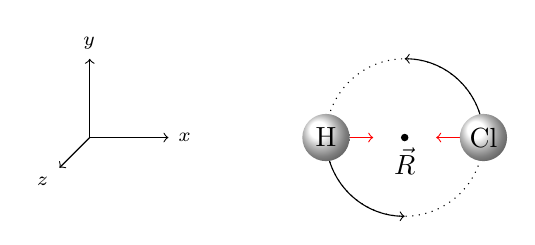
\begin{tikzpicture}
		\coordinate (H) at (1, 0, 0);
		\coordinate (Cl) at (3, 0, 0);

		\draw[->] (-2, 0, 0) -- ++(1, 0, 0) node[right] {$\ev_x$};
		\draw[->] (-2, 0, 0) -- ++(0, 1, 0) node[above] {$\ev_y$};
		\draw[->] (-2, 0, 0) -- ++(0, 0, 1) node[below left] {$\ev_z$};

		\draw[thin, dotted] (Cl) arc (0:360:1);
		\draw[->] (H) arc (180:270:1);
		\draw[->] (Cl) arc (0:90:1);

		\draw[->, color=red] (H) -- ($(H)!.3!(Cl)$);
		\draw[->, color=red] (Cl) -- ($(H)!.7!(Cl)$);

		\shade[ball color=black!.1] (H) circle (3mm) node {H};
		\shade[ball color=yellow!.1] (Cl) circle (3mm) node {Cl};

		\draw[fill] (2, 0, 0) circle (.4mm) node[below] {$\vec R$};
	\end{tikzpicture}
	\caption{%
		Bewegung in einer Ebene. Die anziehende Kraft (rot) hält die Bewegung
		in dieser Ebene.
	}
	\label{fig:3a-Ebene}
\end{figure}

\begin{figure}
	\centering
	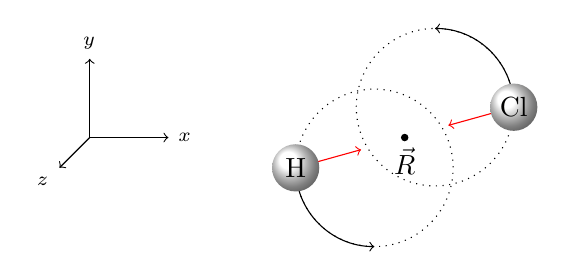
\begin{tikzpicture}
		\coordinate (H) at (1, 0, 1);
		\coordinate (Cl) at (3, 0, -1);

		\draw[->] (-2, 0, 0) -- ++(1, 0, 0) node[right] {$\ev_x$};
		\draw[->] (-2, 0, 0) -- ++(0, 1, 0) node[above] {$\ev_y$};
		\draw[->] (-2, 0, 0) -- ++(0, 0, 1) node[below left] {$\ev_z$};

		\draw[thin, dotted] (Cl) arc (0:360:1);
		\draw[thin, dotted] (H) arc (180:-180:1);
		\draw[->] (H) arc (180:270:1);
		\draw[->] (Cl) arc (0:90:1);

		\draw[->, color=red] (H) -- ($(H)!.3!(Cl)$);
		\draw[->, color=red] (Cl) -- ($(H)!.7!(Cl)$);

		\shade[ball color=black!.1] (H) circle (3mm) node {H};
		\shade[ball color=yellow!.1] (Cl) circle (3mm) node {Cl};

		\draw[fill] (2, 0, 0) circle (.4mm) node[below] {$\vec R$};
	\end{tikzpicture}
	\caption{%
		Bewegung in zwei Ebenen. Die anziehende Kraft (rot) zieht die Teilchen
		aus ihren Ebenen heraus. Dies ist so nicht stabil.
	}
	\label{fig:3a-Ebene}
\end{figure}

%%%%%%%%%%%%%%%%%%%%%%%%%%%%%%%%%%%%%%%%%%%%%%%%%%%%%%%%%%%%%%%%%%%%%%%%%%%%%%%
%              Einstein-Modell der Licht-Materie-Wechselwirkung               %
%%%%%%%%%%%%%%%%%%%%%%%%%%%%%%%%%%%%%%%%%%%%%%%%%%%%%%%%%%%%%%%%%%%%%%%%%%%%%%%

\section{Einstein-Modell der Licht-Materie-Wechselwirkung}
\label 4

\subsection{QED-Prozesse}

Der Term $\textcircled 1$ trägt positiv zur Bilanz bei, es ist also die
Absorption. Je mehr Energie vorhanden ist, und desto mehr Atome im Grundzustand
sind, desto mehr Atome werden angeregt.

Term $\textcircled 2$ hängt noch von der Energiedichte ab, jedoch von der
Anzahl der angeregten Zustände. Außerdem trägt er negativ zur Bilanz bei, so
dass es die stimulierte Emission ist.

Term $\textcircled 3$ ist die spontane Emission, da hier nur die Anzahl der
angeregten Zustände drin ist, und der Term negativ eingeht.

\subsection{Einsteinkoeffizienten}

Im Gleichgewichtsfall mit $\dot N_a = \dot N_g = 0$ werden die beiden Differentialgleichungen zu einer Differentialgleichung:
\begin{align*}
	A N_e &= B \varrho \del{N_g - N_e} \\
	\frac AB &= \varrho \frac{N_g - N_e}{N_e} \\
	\frac AB &= \varrho \del{\frac{N_g}{N_e} - 1} \\
	\frac AB \frac 1\varrho &= \frac{N_g}{N_e} - 1 \\
	\intertext{%
		Da es sich um einen Zustand im thermischen Gleichgewicht handelt, kann
		die Verteilung auch durch die Boltzmann-Verteilung angegeben werden.
		Die Energiedifferenz zwischen den beiden Zuständen ist $\Deltaup E = h
		\nu$. \cite{wikipedia/Einsteinkoeffizienten}
	}
	\frac AB \frac 1\varrho &= \exp\del{\frac{h\nu}{k_\text{B} T}} - 1 \\
	\frac AB \frac{c^3}{8\piup h \nu^3} \del{\exp\del{\frac{h\nu}{k_\text{B} T}} - 1} &= \exp\del{\frac{h\nu}{k_\text{B} T}} - 1 \\
	\frac AB \frac{c^3}{8\piup h \nu^3} &= 1 \\
	\frac AB &= \frac{8\piup h \nu^3}{c^3}
\end{align*}

Dies hängt nicht mehr von der Temperatur ab.

%%%%%%%%%%%%%%%%%%%%%%%%%%%%%%%%%%%%%%%%%%%%%%%%%%%%%%%%%%%%%%%%%%%%%%%%%%%%%%%
%                                    Ende                                     %
%%%%%%%%%%%%%%%%%%%%%%%%%%%%%%%%%%%%%%%%%%%%%%%%%%%%%%%%%%%%%%%%%%%%%%%%%%%%%%%

\IfFileExists{\bibliographyfile}{
	\bibliography{\bibliographyfile}
}{}

\end{document}

% vim: spell spelllang=de
